\smalltitle{سوال 3}
\begin{latin}
    \noindent
    We have two players, so the player space would be $N = \{p_1,p_2\}$ \\
    The action set for player i, Ai would be $a = \text{interval of } (0,1) $ \\
    For player i, the utility function would be $U_i = \frac{f(x_1,x_2)}{2} - c(x_i)$ \\
    We should now, find the inteval in which both players payoffs are equal or greater than zero

\begin{enumerate}
    \item  \phantom{text} \begin{center}
        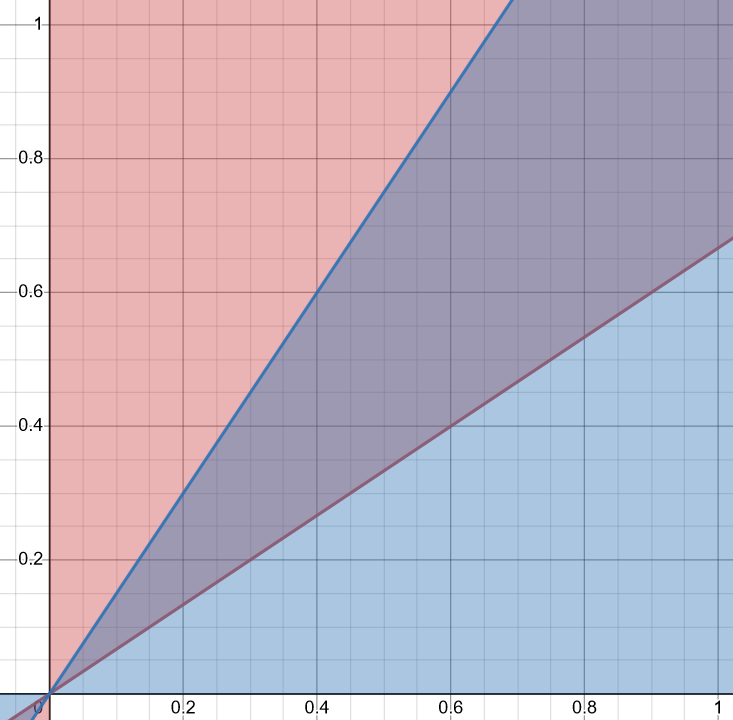
\includegraphics[scale=0.3]{pics/graph1.png} 
        
    \end{center}
    As you could see, the intersection of the blue and red area is the place the game would take place(both payoffs are higher or equal to zero).\\
    If player 1, chooses 0 to work, then the utilities would be : $U_1 = 0$ and $U_2 = -x_2$ so then playet 2 
    would also choose 0 to work. \\
    So if player 1, plays $x_1$, player two would play $\text{argmax } \frac{3}{2}x_1x_2 - x_2^2$ which would be $x_2 = \frac{3x_1}{4}$
    and player 1s payoff would be $\frac{9 * x_1^2}{8} - x_1^2 = \frac{ x_1^2}{8}$. \\
    We know that in interval of (0,1) player 1s payoff is strictly ascending so player 1s best choice would be to choose : 1\\
    So the best moves are when player 1 has move $\frac{3}{4} * x_2 $ and player 2 has $\frac{3}{4} * x_1$ so this goes until both are 0
    so nash equillibrium happens in point (0,0)
    \item  \phantom{text} \begin{center}
        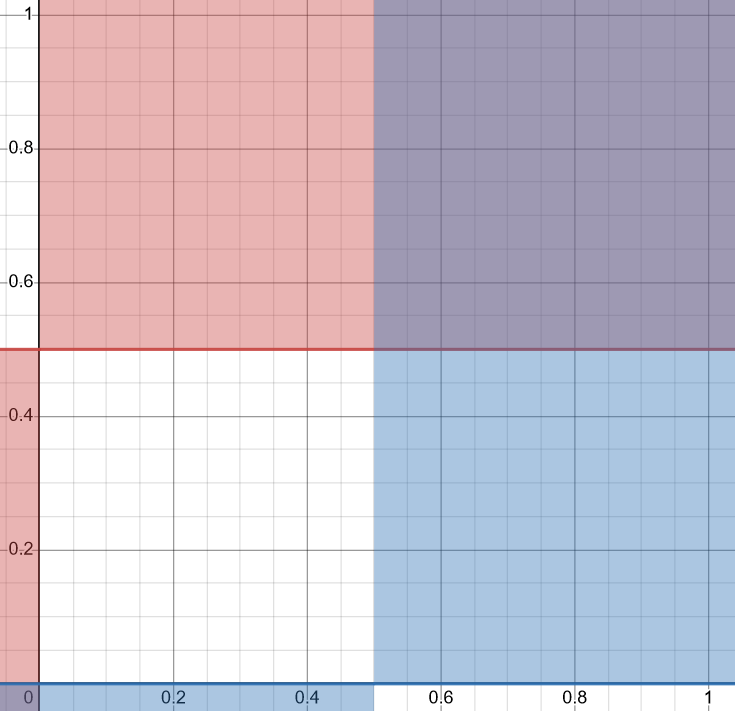
\includegraphics[scale=0.3]{pics/graph2.png} 
        
    \end{center}
    As you could see, the intersection of the blue and red area is the place the game would take place(both payoffs are higher or equal to zero).\\
    If player 1, plays $x_1$ then player 2 would play $\text{argmax } \frac{4}{2}x_1x_2 - x_2$ which would depend on $x_1$ : \\
    $ \begin{cases}
        x_1 > \frac{1}{2} & x_2 = 1 \\
        x_1 \leq \frac{1}{2} & x_2 = 0
    \end{cases} $
     \\
     Then the payoff of player 1 would be : \\
     $ \begin{cases}
        x_1 > \frac{1}{2} & x_1 \\
        x_1 \leq \frac{1}{2} & -x_1
    \end{cases} $ \\
    We see that for player 1, it is best to choose 1 and also for player 2 it is best to choose 1 so the nash equillibrium would be in strategy (1,1)
\end{enumerate}
\end{latin}